%%%%%%%%%%%%%%%%%%%%%%%%%%%%%%%%%%%%%%%%%%%%%%%%%%%%%%%%%%%%%%%%%%%%%%%%%
% This file is part of the LaTeX sources of the OMDoc 1.6 specification
% Copyright (c) 2015 Michael Kohlhase
% This work is licensed by the Creative Commons Share-Alike license
% see http://creativecommons.org/licenses/by-sa/2.5/ for details
% The source original is at https://github.com/KWARC/OMDoc/doc/spec 
%%%%%%%%%%%%%%%%%%%%%%%%%%%%%%%%%%%%%%%%%%%%%%%%%%%%%%%%%%%%%%%%%%%%%%%%%

\begin{omgroup}[creators=miko,id=spec-intro]{The \omdoc Format}

In this chapter we will discuss issues that pertain to the general setup of the \omdoc
format, before we present the respective modules in later chapters. {\omdocv{1.6}} is the
first step towards a second version of the \omdoc format.


\begin{omgroup}[id=syntax-semantics]{Dimensions of Representation in \omdoc}
\begin{newpart}{re-read and strengthen the argumentation}
\begin{wrapfigure}r{8.5cm}\vspace*{-1em}
\fbox{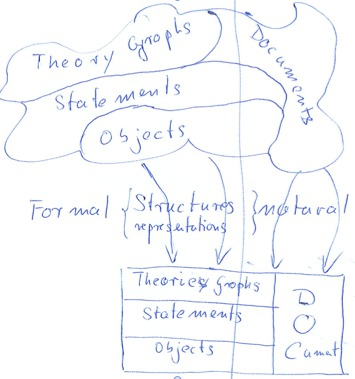
\includegraphics[width=8.2cm]{../figures/omdoc-dimensions}}
\caption{Dimensions of Representation in \omdoc}\label{fig:dimensions}\vspace*{-1em}
\end{wrapfigure}
\paragraph{Strict vs. Pragmatic} The \omdoc format is divided into two sub-languages:
``Strict'' \omdoc (in the lower half of Figure~\ref{fig:dimensions}) and ``Pragmatic''
\omdoc (in the upper half\ednote{add the words ``strict'' and ``pragmatic'' to the
  picture}). The first subset uses a minimal set of elements representing the meaning of a
mathematical expression in a uniform structure, while the second one tries to strike a
pragmatic balance between verbosity and formality. Both forms of content expressions are
legitimate and have their role in representing mathematics. The strict \omdoc format
features a minimal set of conceptually orthogonal representational primitives, resulting
in expressions with canonical structure, which simplifies the implementation of \omdoc
processors as well as the comparison of content expressions.  The pragmatic \omdoc
format provides a large representational infrastructure that aims at being intuitive for
humans to understand, read, and write.\ednote{maybe state the numbers of elements in the
  end} In particular, the simplicity and conceptual clarity of strict \omdoc allow to
express structural well-formedness constraints, whereas the vocabulary of pragmatic \omdoc
is much nearer to mathematical practice and is thus easier to learn. It is a crucial
design choice of the \omdoc format that the meaning fo pragmatic representations is
defined entirely interms of strict representations\footnote{The strategy of dividing a
  markup format into a simple and structurally elegant core language and a larger set of
  pragmatic extensions which can be given a meaning by translating into the core was first
  pioneered by the author for content {\mathml}3~\cite{CarlisleEd:MathML3}}. Note that
there may be multiple ``pragmatic vocabularies'' defined in terms of the strict core
catering to different communities and their tastes.

The introduction of strict \omdoc and the re-interpretation of pragmatic \omdoc in
terms of it is radical redesign of the \omdoc format, which is new in {\omdocv{1.6}}.
For this reason we consider {\omdocv{1.6}} the first step into the directiosn of
{\omdocv{2}}. With the development of strict \omdoc we aim to identify the
representational primitives for representing mathematical documents, which can be given a
simple and elegant semantics.

\paragraph{Formal vs. Informal} 

One of the hallmarks of mathematical language is that it is very rigorous in structure and
usage in an attempt to fix the meaning of (mathematical) objects and statements about
them. Indeed, the first decades of the last century established that mathematical language
can in principle be expanded into logical form, where all objects and statements are fully
identified by their syntactic form, and all reasoning steps are similarly justified by
their form alone. we speak of ``formal mathematics'', when this is exercised and of
``formal reasoning'', when proofs are carried out in logical systems on this basis . In
the last decades, significant parts of mathematical knowledge have been formalized and
verified with the help of computers. But formalization and formal reasoning is still so
costly and tedious that only a very small part of mathematics is formalized and verified
in practice. Currently almost all mathematical documents consist of a mix of formal and
informal (i.e. natural language) elements --- certainly during the development of
mathematical knowledge, but also in publications. Therefore representation formats for
mathematical documents must allow this as well, consequently, \omdoc has two
sub-languages, ``formal \omdoc'' (on the left side of Figure~\ref{fig:dimensions}) and
``natural \omdoc'' (on the right side).

\omdoc offers markup at three levels: objects, statements, and context.
\begin{compactdesc}
\item[objects] are usually represented as {\emph{formulae}} or \emph{natural language
    phrases} in mathematical documents. In formal \omdoc formulae are marked up according
  to their functional structure (as operator trees) and according to their layout in
  informal \omdoc (as layout trees). Note that any object can be represented in both ways
  and both ways of representation can be mixed at any level to account for mathematical
  practice, e.g. for mixed formulae like $\{n\in\mathbb{N}\bigl|\text{$n$ is prime and
    $n>2$}\}$.
\item[statements] are usually represented as \emph{natural language sentences (with
    formulae)}\footnote{or even larger text fragments made up of sentences like
    paragraphs} in informal settings and as (closed, logical) formulae in formal ones. The
  discussion about the two ways of representation of objects applies analogously. Note
  that functional markup in formal \omdoc only addresses part of the requirements of
  formality, since their meaning depends on their context; we will explore this next.
\item[theory graphs] The context of objects (and the statements that contain them) is
  given by special statements (declarations). For conciseness and tractability, \omdoc
  groups declarations into ``theories'' and connects them by ``theory morphisms'' into
  ``theory graphs''. In a nutshell, every object (and thus every statement) has a ``home
  theory'', in which it is meaningful. Theory morphisms make objects and statements
  available in their target theories.
\end{compactdesc}
As statements, theories and theory graphs are large objects, their informal
representations (as mathematical text fragments and documents) usually carry linguistic
cues to their discourse structure\ednote{change the ``documents'' in
  Figure~\ref{fig:dimensions} to ``discourse'', at least in the strict box}. We discuss
the relation between the discourse structure of informal representations and the formal
structure of statements and theory graphs next.

\paragraph{Discourse vs. Content Structure}

Mathematical documents are very explicitly structured to help the reader grasp the complex
objects, their relationships, and the flow of the argumentation in the proofs: Objects are
often represented as formulae that reveal their structure, statements are labeled by
indicators to their epistemic contribution to context (e.g. by labeling them as
``definitions'' or ``theorems'') and numbered for exact reference. The exposition of
larger documents usually follows a topical structure with superimposed narrative structure
driven by knowledge dependencies rather than e.g. a temporal dramaturgy driven by
suspense.  Even so, the structure of an informal document may be quite different from the
formal structure of the knowledge it introduces.

\begin{wrapfigure}l{7cm}\vspace*{-2em}
  \infigures{content_vs_narrative}
\caption{Content vs. Narrative Structures}\label{fig:straw-man}
\end{wrapfigure}
For instance, when we introduce a new concept in a course, we often first introduce a
naive reduced approximation $\mathcal{N}$ of the real theory $\mathcal{F}$, only to show
an example $\mathcal{E_N}$ of where this is insufficient. Then we propose a first
(straw-man) solution $\mathcal{S}$, and show an example $\mathcal{E_S}$ of why this does
not work. Based on the information we gleaned from this failed attempt, we build the
eventual version $\mathcal{F}$ of the concept or theory and demonstrate that this works on
$\mathcal{E_F}$.
 
The structure with the solid lines and boxes at the bottom of {\myfigref{straw-man}}
represents the content structure, where the circles $\mathcal{N}$, $\mathcal{E_N}$,
$\mathcal{S}$, $\mathcal{E_S}$, $\mathcal{F}$, and $\mathcal{E_F}$ signify theories for
the content of the respective concepts and examples. The arrows represent the
{\twintoo{theory}{inheritance}} structure, e.g. Theory $\mathcal{F}$ imports theory
$\mathcal{N}$. The top part of the diagram with the dashed lines stands for the narrative
structure, where the arrows mark up the document structure. For instance, the slides
$\text{sl}_i$ are grouped into a lecture. In the example in {\myfigref{straw-man}}, the
second slide of ``lecture'' presents the first example: the text fragment $\text{n}_1$
introduces it, and $\text{n}_2$ presents $\mathcal{E_N}$ and $\text{n}_2$ might say
something like ``this did not work in the current situation, so we have to extend the
conceptualization\ldots''. In a conventional setting, the narrative structure on the top
and the content structure would be represented in different documents: The lecture slides
and the formalization, and the equivalences (e.g. that $\text{n}_2$ verbalizes
$\mathcal{E_N}$; we have visualized these relations as dotted arrows in
{\myfigref{straw-man}}) could not be taken advantage of, since they are not explicitly
represented.

\begin{wrapfigure}r{7.5cm}\vspace*{-1em}
\infigures{adp}
\caption{The Active Documents Paradigm}\label{fig:adp}\vspace*{-1em}
\end{wrapfigure}
But these equivalences can be utilized to render services to the reader, for instance the
imports relation in the theory graph on the lower half of Figure~\ref{fig:straw-man}
induces a dependency relation that can be used to generate a minimal explanation (without
the motivation) of $\cE_\cF$.  For an example at the object level, consider for instance
the formula $a(x+y^2)$, whose layout is ambiguous in two places: $a$ could be a factor in
a product (presented as juxtaposition) or a function that is applied to an
argument. Likewise $y^2$ could be the variable $y$ raised to the second power or the
second element in the sequence $y^1,y^2,\ldots,y^n$. Humans can usually disambiguate this
from the context, but a screen reader service needs access to the operator tree to read
this as ``$a$ times [pause] $x$ plus $y$ squared'' or ``$a$ applied to [pause] $x$ plus
$y$ two''.

\omdoc aims to reconcile the dichotomy between discourse structures (in informal
mathematical documents which currently carry most of mathematical knowledge) and formal
structures (that machines can operate upon) in one joint format. The central technique
employed in \omdoc is that of ``parallel markup'': The technique comes from MathML, where
the \element{semantics} element is used to accomodate equivalent layout (presentation
{\mathml}) and operator trees (content {\mathml}) and possibly foreign
representations. Equivalence of nested sub-structures are represented by special
cross-references.  The \mathml processor choses the one most adequate to its task --- in
the absence of distinguisthing information the first child.

\omdoc extends this to the document level: The document contains elements whose children
are alternative representations of the same object/statement/theory.\ednote{implement
  this, and think about the cross-referencing, also need continuations to break tree
  overlaps, e.g. in content objects straddling slides.} The significance of this is

for that is Figure~\ref{fig:adp} shows the \ednote{talk about parallel markup, content
  documents and narrative documents and how to crosslink them and share structure}.


Just as for content-based systems on the formula level, there are now MKM systems that
generate presentation markup from content markup, based on general presentation
principles, also on this level. For instance, the {\sc{ActiveMath}}
system~\cite{MelBue:krma03} generates a simple narrative structure (the
presentation; called a personalized book) from the underlying content structure (given in
\omdoc) and a user model.

\paragraph{Coverage} 
Currently our understanding of these primitives is largely limited to formal parts of
mathematics, therefore strict {\omdocv{1.6}} covers significantly less of informal
mathematical documents than {\omdocv{1.2}}, so the meaning-giving translation from
pragmatic \omdoc elements to strict \omdoc is partial. We plan to develop strict
\omdoc into a system with greater coverage in the upcoming versions of \omdoc.
{\omdocv{2.0}} will be the first stable version where the coverage of strict \omdoc is
complete.
\end{newpart}
\end{omgroup}

\begin{omgroup}[id=spec-intro.modular]{\omdoc as a Modular Format}

A modular approach to design is generally accepted as best practice in the development of
any type of complex application. It separates the application's functionality into a
number of "{\indextoo{building blocks}}" or "{\indextoo{module}s}", which are subsequently
combined according to specific rules to form the entire application. This approach offers
numerous advantages: The increased {\indextoo{conceptual clarity}} allows developers to
share ideas and code, and it encourages reuse by creating well-defined modules that
perform a particular task. Modularization also reduces complexity by decomposition of the
application's functionality and thus decreases debugging time by localizing errors due to
design changes. Finally, flexibility and maintainability of the application are increased
because single modules can be upgraded or replaced independently of others.

The \omdoc vocabulary has been split by thematic role, which we will briefly overview in
{\myfigref{omdoc-modules}} before we go into the specifics of the respective modules in
{\srefl{mobj}{quiz}}. To avoid repetition, we will introduce some attributes already in
this chapter that are shared by elements from all modules. In \sref{document-model} we
will discuss the \omdoc document model and possible sub-languages of \omdoc that only
make use of parts of the functionality (\sref{sub-languages}).

\begin{myfig}{omdoc-modules}{The \omdoc Modules}
\begin{small}
\begin{tabular}{|l|l|l|l|}\hline
  Module & Title & Required? & Chapter\\\hline\hline
  {\presbf\MOBJmodule{spec}} &  Mathematical Objects & yes & \sref{mobj}\\\hline
    \multicolumn{4}{|p{11cm}|}{\presem Formulae are a central part of mathematical
       documents; this module integrates the content-oriented representation
       formats {\openmath} and {\mathml} into \omdoc}\\\hline\hline
  {\presbf\MTXTmodule{spec}} &  Mathematical Text & yes & \sref{mtext}\\\hline
    \multicolumn{4}{|p{11cm}|}{\presem Mathematical vernacular,
  i.e. natural language with embedded formulae}\\\hline\hline
  {\presbf\DOCmodule{spec}} & Document Infrastructure & yes & \sref{omdoc-infrastructure}\\\hline
    \multicolumn{4}{|p{11cm}|}{\presem  A basic infrastructure for
      assembling pieces of  mathematical knowledge into functional documents and 
      referencing their parts }\\\hline\hline
  {\presbf\METAmodule{spec}} &  Metadata & yes &   {\srefs{dc-elements}{dc-roles}}\\\hline
    \multicolumn{4}{|p{11cm}|}{\presem Contains bibliographical and licensing metadata 
      (``{\twintoo{data}{about data}}'') 
      which can be used to annotate many \omdoc elements by descriptive and
      administrative information that facilitates navigation and organization}\\\hline\hline 
  {\presbf\RTmodule{spec}} & Rich Text Structure & no & \sref{rt}\\\hline
    \multicolumn{4}{|p{11cm}|}{\presem Rich text structure in
  mathematical vernacular (lists, paragraphs, tables, \ldots)}\\\hline\hline
  {\presbf\STmodule{spec}} &  Mathematical Statements & no  & \sref{statements}\\\hline
    \multicolumn{4}{|p{11cm}|}{\presem Markup for mathematical forms like 
      {\indextoo{theorem}s},  {\indextoo{axiom}s}, {\indextoo{definition}s}, 
      and {\indextoo{example}s} that can be used to specify or define properties
      of given mathematical objects and theories to group mathematical
  statements and provide a notion of context.}\\\hline\hline
  {\presbf\PFmodule{spec}} &  Proofs and proof objects & no & \sref{proofs}\\\hline 
    \multicolumn{4}{|p{11cm}|}{\presem Structure of proofs
     and argumentations at various levels of details and formality}\\\hline\hline
  {\presbf\ADTmodule{spec}} &  Abstract Data Types & no & \sref{adt}\\\hline 
    \multicolumn{4}{|p{11cm}|}{\presem  Definition schemata for
      sets that are built up inductively from constructor symbols}\\\hline\hline 
  {\presbf\CTHmodule{spec}} & Complex Theories & no & \sref{complex-theories}\\\hline
    \multicolumn{4}{|p{11cm}|}{\presem Theory morphisms; they can be used
    to structure mathematical theories}\\\hline\hline
  {\presbf\DGmodule{spec}} & Development Graphs & no & \sref{development-graphs}\\\hline
    \multicolumn{4}{|p{11cm}|}{\presem Infrastructure for managing theory
  inclusions, change management}\\\hline\hline
  {\presbf\EXTmodule{spec}} & Applets, Code, and Data & no & \sref{ext}\\\hline
    \multicolumn{4}{|p{11cm}|}{\presem Markup for applets, program code,
  and data (e.g. images, measurements, \ldots)}\\\hline\hline
  {\presbf\PRESmodule{spec}} & Presentation Information & no &  \sref{pres}\\\hline
    \multicolumn{4}{|p{11cm}|}{\presem Limited functionality for
    specifying presentation and notation information for local typographic
      conventions  that cannot be determined by general principles alone}\\\hline\hline
  {\presbf\QUIZmodule{spec}} &  Infrastructure for Assessments & no & \sref{quiz}\\\hline
    \multicolumn{4}{|p{11cm}|}{\presem Markup for exercises integrated
    into the \omdoc document model}\\\hline 
  \end{tabular}
\end{small}
\end{myfig}
The first four modules in {\myfigref{omdoc-modules}} are required (mathematical documents
without them do not really make sense), the other ones are optional. The
document-structuring elements in module {\DOCmodule{spec}} have an attribute
{\attributeshort{modules}} that allows to specify which of the modules are used in a
particular document (see \sref{omdoc-infrastructure} and
\sref{sub-languages}).
\end{omgroup}

\begin{omgroup}[id=omdoc-ns]{The OMDoc Namespaces}

The namespace for the {\omdocv2} format is the \atwinalt{URI}{OMDoc}{namespace}{URI}
\url{http://omdoc.org/ns}. Note that the \omdoc \twinalt{namespace}{OMDoc}{namespace}
does not reflect the versions\footnote{The namespace is different from the {\omdocv1}
  formats (versions 1.0, 1.1, and 1.2), which was
  {\snippet{http://www.mathweb.org/omdoc}}, but the {\omdocv2} namespace will stay
  constant over all versions of the {\omdocv2} format.}, this is done in the
{\attributeshort{version}} attribute on the {\twintoo{document}{root}} element
\element{omdoc} (see \sref{omdoc-infrastructure}).  As a consequence, the
\omdoc vocabulary identified by this namespace is not static, it can change with each
new \omdoc version. However, if it does, the changes will be documented in later
versions of the specification: the latest released version can be found
at~\cite{URL:omdocspec}.

In an \omdoc document, the \omdoc namespace must be specified either using a
{\twintoo{namespace}{declaration}} of the form
{\snippet{xmlns="}}\url{http://omdoc.org/ns}{\snippet{"}} on the \element{omdoc} element
or by prefixing the {\twintoo{local}{name}s} of the \omdoc elements by a namespace
prefix (\omdoc customarily use the prefixes {\snippet{omdoc:}} or {\snippet{o:}}) that
is declared by a {\atwintoo{namespace}{prefix}{declaration}} of the form
{\snippet{xmlns:o="}}\url{http://omdoc.org/ns}{\snippet{"}} on some element dominating the
\omdoc element in question (see {\extref{book}{xml}} for an introduction). \omdoc also
uses the following namespaces\footnote{In this specification we will use the
  {\twintoo{namespace}{prefix}es} above on all the elements we reference in text unless
  they are in the \omdoc namespace.}:

\begin{scriptsize}
  \begin{center}
    \begin{tabular}{|l|l|l|}\hline
      Format      & namespace URI & see \\\hline\hline
      Dublin Core & \url{http://purl.org/dc/elements/1.1/} &   {\srefs{dc-elements}{dc-roles}}\\\hline
      Creative Commons & \url{http://creativecommons.org/ns} & \sref{creativecommons}\\\hline
      {\mathml} & \url{http://www.w3.org/1998/Math/MathML} & \sref{cmml}\\\hline
      {\openmath} & \url{http://www.openmath.org/OpenMath} & \sref{openmath}\\\hline
      {\xslt} & \url{http://www.w3.org/1999/XSL/Transform} & \sref{pres}\\\hline
    \end{tabular}
  \end{center}
\end{scriptsize}
Thus a typical document root of an \omdoc document looks as follows:
  \begin{lstlisting}[mathescape]
<?xml version="1.0" encoding="utf-8"?>
<omdoc xml:id="test.omdoc" version="1.6"
  xmlns="http://omdoc.org/ns"
  xmlns:cc="http://creativecommons.org/ns"
  xmlns:dc="http://purl.org/dc/elements/1.1/"
  xmlns:om="http://www.openmath.org/OpenMath"
  xmlns:m="http://www.w3.org/1998/Math/MathML">
$\ldots$
</omdoc>
\end{lstlisting}  
\end{omgroup}

\begin{omgroup}[id=common-attribs]{Common Attributes in OMDoc}

Generally, the \omdoc format allows any attributes from foreign (i.e. non-\omdoc)
\twinalt{namespaces}{foreign}{namespace} on the \omdoc elements. This is a commonly
found feature that makes the {\xml} encoding of the \omdoc format extensible. Note
that the attributes defined in this specification are in the default (empty)
\twinalt{namespace}{default}{namespace}: they do not carry a namespace prefix. So any
attribute of the form {\snippet{na:xxx}} is allowed as long as it is in the scope of a
suitable {\atwintoo{namespace}{prefix}{declaration}}.

Many \omdoc elements have optional {\attributeshort[ns-attr=xml]{id}} attributes that
can be used as identifiers to reference them. These attributes are of type
\twinalt{\snippet{ID}}{type}{ID}, they must be unique in the document which is important,
since many {\xml} \twinalt{applications}{XML}{application} offer functionality for
referencing and retrieving elements by \twinalt{{\snippet{ID}}-type}{type}{ID} attributes.
Note that unlike other {\snippet{ID}}-attributes, in this special case it is the name
{\attributeshort[ns-attr=xml]{id}}~\cite{XML:id05} that defines the
{\indextoo{referencing}} and {\indextoo{uniqueness}} functionality, not the type
declaration in the {\indextoo{DTD}} or {\twintoo{XML}{schema}} (see
{\extref{book}{xml.validation}} for a discussion).

  Note that in the \omdoc format proper, all {\twintoo{ID}{type}} attributes are of the
  form {\attributeshort[ns-attr=xml]{id}}. However in the older {\openmath} and {\mathml}
  standards, they still have the form {\attributeshort{id}}. The latter are only
  recognized to be of type {\snippet{ID}}, if a document type or {\xml}schema is
  present. Therefore it depends on the application context, whether a DTD should be
  supplied with the \omdoc document.

  For many occasions (e.g. for printing \omdoc documents), authors want to control a
  wide variety of aspects of the presentation. \omdoc is a content-oriented format, and
  as such only supplies an infrastructure to mark up content-relevant information in
  \omdoc elements. To address this dilemma {\xml} offers an interface to 
  {\twintoo{Cascading}{Style Sheet}s} ({\css})~\cite{BosHak:css98}, which allow to specify
  presentational traits like {\twintoo{text}{color}}, {\twintoo{font}{variant}},
  {\indextoo{positioning}}, {\indextoo{padding}}, or {\indextoo{frame}s} of
  {\twintoo{layout}{box}es}, and even {\indextoo{aural}} aspects of the text.

  To make use of {\css}, most \omdoc elements (all that have
  {\attributeshort[ns-attr=xml]{id}} attributes) have {\attributeshort{style}} attributes
  that can be used to specify {\css} \twinalt{directives}{CSS}{directive} for them. In the
  \omdoc fragment in {\mylstref{css-basic}} we have used the \attribute{style}{omtext}
  attribute to specify that the text content of the \element{omtext} element should be
  formatted in a centered box whose width is 80\% of the surrounding box (probably the
  page box), and that has a 2 pixel wide solid frame of the specified RGB color. Generally
  {\css} directives are of the form {\snippet{A:V}}, where {\snippet{A}} is the name of
  the aspect, and {\snippet{V}} is the value, several {\css}
  \twinalt{directives}{CSS}{directive} can be combined in one {\attributeshort{style}}
  attribute as a {\twintoo{semicolon-separated}{list}} (see {\cite{BosHak:css98} and the
    emerging {\css} 3} standard).

\begin{lstlisting}[label=lst:css-basic,mathescape,
   caption={Basic {\css} Directives in a {\attributeshort{style}} Attribute},
   index={style,class}]
<?xml version="1.0" encoding="utf-8"?>
<?xml-stylesheet type="text/css" href="http://example.org/style.css"?>
<omdoc xml:id="stylish">
  $\ldots$
  <omtext xml:id="t1" style="width:80%;align:center;border:2px #006699 solid">
    <h:p>Here comes something 
      <h:span style="font-weight:bold;color:green" class="emphasize">stylish</h:span>!
    </h:p>
  </omtext>
  $\ldots$
</omdoc>
\end{lstlisting}

Note that many {\css} properties of parent elements are inherited by the children,
if they are not explicitly specified in the child. We could for instance have set
the {\twintoo{font}{family}} of all the children of the \element{omtext} element
by adding a directive {\snippet{font-family:sans-serif}} there and then override it by
a directive for the property {\snippet{font-family}} in one of the children.

Frequently recurring groups of {\css} directives can be given symbolic names in {\css}
\twinalt{styles heets}{CSS}{style sheet}, which can be referenced by the
{\attributeshort{class}} attribute. In {\mylstref{css-basic}} we have made use of this
with the class {\snippet{emphasize}}, which we assume to be defined in the style sheet
{\snippet{style.css}} associated with the document in the ``{\twintoo{style
    sheet}{processing instruction}}'' in the prolog\footnote{i.e. at the very beginning of
  the {\xml} document before the document type declaration} of the {\xml} document
(see~\cite{Clark:assxd99} for details).  Note that an \omdoc element can have both
{\attributeshort{class}} and {\attributeshort{style}} attributes, in this case, precedence
is determined by the rules for {\css} style sheets as specified in~\cite{BosHak:css98}. In
our example in {\mylstref{css-basic}} the directives in the {\attributeshort{style}}
attribute take precedence over the {\css} directives in the style sheet referenced by the
{\attributeshort{class}} attribute on the \element{phrase} element. As a consequence,
the word ``stylish'' would appear in green, bold italics.
\end{omgroup}
%%%%%%%%%%%%%%%%%%%%%%%%%%%%%%%%%%%%%%%%%%%%%%%%%%%%%%%%%%%%%%%%%%%%%%%%%
% This file is part of the LaTeX sources of the OMDoc 1.6 specification
% Copyright (c) 2006 Michael Kohlhase
% This work is licensed by the Creative Commons Share-Alike license
% see http://creativecommons.org/licenses/by-sa/2.5/ for details
% The source original is at https://github.com/KWARC/OMDoc/doc/spec 
%%%%%%%%%%%%%%%%%%%%%%%%%%%%%%%%%%%%%%%%%%%%%%%%%%%%%%%%%%%%%%%%%%%%%%%%%

\begin{module}[id=genmeta]
\begin{omgroup}[creators={miko,clange},short={Metadata},id=metadatachap]
  {Metadata (Module {\METAmodule{spec}})}

\begin{newpart}{@CL, please re-read and expand}
  \indexalt{Metadata}{metadata} is ``{\twintoo{data}{about data}}'' --- in the case of
  \omdoc data about documents fragments, such as titles, authorship, language usage, or
  administrative aspects like modification dates, distribution rights, identifiers, or
  version information. \omdoc documents also contain data about realations between
  mathematical objects, statements, and theories, that other applications would consider
  as metadata. To ensure interoperability with such applications and the Semantic Web,
  \omdoc supports the extraction of \omdoc-specific metadata to the RDF
  format\ednote{MK@CL write up something about processing in projects or processing and
    reference it here} and the annotation of many \omdoc elements with web-ontology
  metadata.

  In this section we will introduce the metadata framework for {\twintoo{strict}{omdoc}},
  which provides a generic, extensible infrastructure for adding metadata based on the
  recently stabilized RDFa~\cite{AdidaEtAl08:RDFa} a standard for flexibly embedding
  metadata into X(HT)ML documents. This design decision allows us to separate the
  {\emph{syntax}} (which is standardized in RDFa) from the {\emph{semantics}}, which we
  externalize in metadata ontologies, which can be encoded in \omdoc; see
  {\extref{primer}{ontology}}.



\begin{omtext}
  The \omdoc format will incorporate various concrete metadata vocabularies as part of
  the document format. These are given as documented ontologies encoded as \omdoc
  theories and are normative parts of the format specification. Note that these metadata
  theories\ednote{MK@MK: reference theory framework (probably the strict one)} can be
  thought of as the minimal specifications of the metadata: Refinements are admissible, if
  they are formulated as \omdoc theories that entertain views into the normative
  theories.\ednote{MK@MK: dream up a framework how to include the ontologies into the spec
    (probably as the DC and CC chapters; but do not forget the assertion type ontology,
    see \tracticket{1511}).}
\end{omtext}

\begin{myfig}{qtmetadata}{Metadata in \omdoc}
  \begin{scriptsize}
\begin{tabular}{|>{\tt}l|>{\tt}l|>{\tt}l|>{\tt}l|}\hline
{\rm Element}& \multicolumn{2}{l|}{Attributes\hspace*{2.25cm}} & Content  \\\hline
                 & {\rm Req.}  & {\rm Optional}   &           \\\hline\hline
metadata  &             &                     &  (meta|link)*\\\hline
meta         & property,content         &  datatype               & ANY \\\hline
link           & rel & href & (resource|mlink|meta)*\\\hline
resource   & & typeof, about & (meta|link)*\\\hline
\end{tabular}
\end{scriptsize}
\end{myfig}

\begin{definition}[id=metadata.def]
  The {\eldef{metadta}} element contains content encodings for RDF triples and
  resources. \ednote{@CL: need to verbalize this.}
\end{definition}
\ednote{@CL: explain curies here.}  
\ednote{@CL: need a simple example here, best DC  metadata that we can take up later. }

\begin{omgroup}{Pragmatic to Strict Translation}
  Every \omdoc element that admits a \element{metadata} child can serve as a metadata
  subject, so we can offer the following pragmatic (abbreviative) syntax:
\begin{center}\lstset{frame=none,numbers=none,lineskip=-.7ex,aboveskip=-.5em,belowskip=-1em,mathescape}
 \begin{tabular}{|p{5cm}|p{5cm}|}\hline
    pragmatic & strict equivalent\\\hline
\begin{lstlisting}
<$\llquote{elt}$ rel="$\llquote{r}$" href="$\llquote{h}$">
  $\llquote{body}$
</$\llquote{elt}$>
\end{lstlisting}
&
\begin{lstlisting}
<$\llquote{elt}$>
  <metadata>
    <link rel="$\llquote{r}$" href="$\llquote{h}$"/>
  </metadata>
  $\llquote{body}$
</$\llquote{elt}$>
\end{lstlisting}
\\\hline 
\begin{lstlisting}
<$\llquote{elt}$ rel="$\llquote{r}$" href="$\llquote{h}$">
  <metadata>
   $\llquote{meta}$
  </metadata>
  $\llquote{body}$
</$\llquote{elt}$>
\end{lstlisting}
&
\begin{lstlisting}
<$\llquote{elt}$>
  <metadata>
    <link rel="$\llquote{r}$" href="$\llquote{h}$"/>
    $\llquote{meta}$
 </metadata>
  $\llquote{body}$
</$\llquote{elt}$>
\end{lstlisting}
\\\hline 
\end{tabular}
\end{center}
\end{omgroup}


{\omdocv{1.2}} had some descriptions of metadata inhertance for Dublin Core Metadata. In
the new metadata framework we do not need to explicitly present this, since it is part of
the metadata ontology: If a metadatum can be inferred it is defined to be
present. \ednote{@CL, make a simple concrete example.}
\end{newpart}
\end{omgroup}
\end{module}

%%% Local Variables: 
%%% mode: latex
%%% TeX-master: "main"
%%% End: 


%%%%%%%%%%%%%%%%%%%%%%%%%%%%%%%%%%%%%%%%%%%%%%%%%%%%%%%%%%%%%%%%%%%%%%%%%
% This file is part of the LaTeX sources of the OMDoc 1.6 specification
% Copyright (c) 2006 Michael Kohlhase
% This work is licensed by the Creative Commons Share-Alike license
% see http://creativecommons.org/licenses/by-sa/2.5/ for details
% The source original is at https://github.com/KWARC/OMDoc/doc/spec 
%%%%%%%%%%%%%%%%%%%%%%%%%%%%%%%%%%%%%%%%%%%%%%%%%%%%%%%%%%%%%%%%%%%%%%%%%

\begin{module}[id=dc-elements]
  \begin{omgroup}[id=dc-elements]{Dublin Core Metadata in \omdoc}

The most commonly used metadata standard is the Dublin Core vocabulary, which is
supported in some form by most formats. \omdoc uses this vocabulary for compatibility
with other metadata applications and extends it for {\twintoo{document}{management}}
purposes in \omdoc.  Most importantly \omdoc extends the use of metadata from
documents to other (even mathematical) elements and {\twintoo{document}{fragment}s} to
ensure a fine-grained authorship and {\twintoo{rights}{management}}.


\begin{newpart}{MK@CL, please discuss}
\begin{omgroup}{Dublin Core Ontology}

\end{omgroup}

\begin{omgroup}{Pragmatic Dublin Core Elements}

In the following we will describe the variant of Dublin Core metadata elements used in
\omdoc.  Here, the \element{metadata} element can contain any number of instances of
any Dublin Core elements described below in any order. In fact, multiple instances of the
same element type (multiple \element[ns-elt=dc]{creator} elements for example) can be
interspersed with other elements without change of meaning.  \omdoc extends the Dublin
Core framework with a set of roles (from the MARC relator set~\cite{Marc:relators03}) on
the authorship elements and with a rights management system based on the Creative Commons
Initiative.


The descriptions in this section are adapted from~\cite{DCMI:dmt03}, and augmented for the
application in \omdoc where necessary. All these elements live in the {\twintoo{Dublin
    Core}{namespace}} \url{http://purl.org/dc/elements/1.1/}, for which we traditionally
use the {\twintoo{namespace}{prefix}}\atwinalt {\snippetin{dc:}}{Dublin
  Core}{namespace}{URI}.
\begin{myfig}{qtdc}{Dublin Core Metadata in \omdoc}
  \begin{scriptsize}
\begin{tabular}{|>{\tt}l|>{\tt}l|>{\tt}l|>{\tt}l|}\hline
{\rm Element}& \multicolumn{2}{l|}{Attributes\hspace*{2.25cm}} & Content  \\\hline
             & {\rm Req.}  & {\rm Optional}     &           \\\hline\hline
 dc:creator     &  & xml:id, class, style, role    &  ANY \\\hline
 dc:contributor &  & xml:id, class, style, role    &  ANY\\\hline
 dc:title       &  & xml:lang    &  \llquote{math vernacular}  \\\hline
 dc:subject     &  & xml:lang    &  \llquote{math vernacular}  \\\hline
 dc:description &  & xml:lang    &  \llquote{math vernacular}  \\\hline
 dc:publisher   &  & xml:id, class, style          &  ANY  \\\hline
 dc:date        &  & action, who &  {\twintoo{ISO}{8601}}  \\\hline
 dc:type        &  &             &  {\rm fixed:} "Dataset" {\rm or\ } "Text" \\\hline
 dc:format      &  &             &  {\rm fixed:} "application/omdoc+xml"  \\\hline
 dc:identifier  &  & scheme      &  ANY  \\\hline
 dc:source      &  &             &  ANY  \\\hline
 dc:language    &  &             &  {\twintoo{ISO}{639}} \\\hline
 dc:relation    &  &             &  ANY  \\\hline
 dc:rights      &  &             &  ANY  \\\hline\hline
 \multicolumn{4}{|l|}{for \llquote{math vernacular} see \sref{mtext}}\\\hline
\end{tabular}
\end{scriptsize}
\end{myfig}

\begin{definition}[id=dc.title.def,title=Titles]
  The title of the element --- note that \omdoc metadata can be specified at multiple
  levels, not only at the document level, in particular, the Dublin Core
  {\eldef[ns-elt=dc]{title}} element can be given to assign a title to a theorem, e.g. the
  ``Substitution Value Theorem''.
  
  The \element[ns-elt=dc]{title} element can contain
  {\twintoo{mathematical}{vernacular}} (see \sref{mtext}). Multiple
  \element[ns-elt=dc]{title} elements inside a \element{metadata} element are assumed
  to be translations of each other.\ednote{do we still want this?}
\end{definition}

\begin{definition}[id=dc.creator.def,title=Creators]
  A primary creator or author of the publication.  Additional contributors whose
  contributions are secondary to those listed in {\eldef[ns-elt=dc]{creator}} elements
  should be named in \element[ns-elt=dc]{contributor} elements.  Documents with multiple
  co-authors should provide multiple \element[ns-elt=dc]{creator} elements, each
  containing one author.  The order of \element[ns-elt=dc]{creator} elements is presumed
  to define the order in which the creators' names should be presented.
  
  As markup for names across cultures is still un-standardized, \omdoc recommends that
  the content of a \element[ns-elt=dc]{creator} element consists in a single name (as it
  would be presented to the user). The \element[ns-elt=dc]{creator} element has an
  optional attribute \attribute[ns-elt=xml,ns-attr=dc]{id}{creator} so that it can be
  {\indextoo{cross-reference}d} and a {\attributeshort{role}} attribute to further
  classify the concrete contribution to the element. We will discuss its values in
  \sref{dc-roles}.
\end{definition}

\begin{definition}[id=dc.contributor.def,title=Contributors]
  A party whose contribution to the publication is secondary to those named in
  \element[ns-elt=dc]{creator} elements.  Apart from the significance of contribution,
  the semantics of the {\eldef[ns-elt=dc]{contributor}} is identical to that of
  \element[ns-elt=dc]{creator}, it has the same restriction content and carries the same
  attributes plus a \attribute[ns-elt=xml,ns-attr=dc]{lang}{contributor} attribute that
  specifies the target language in case the contribution is a translation.
\end{definition}

\begin{definition}[id=dc.subject.def,title=Subjects]
  This element contains an arbitrary phrase or keyword, the attribute
  \attribute[ns-elt=xml,ns-attr=dc]{lang}{subject} is used for the language. Multiple
  instances of the {\eldef[ns-elt=dc]{subject}} element are supported per
  \attribute[ns-elt=xml,ns-attr=dc]{lang}{subject} for multiple keywords.
\end{definition}

\begin{definition}[id=dc.description.def,title=Descriptions]
  A text describing the containing element's content; the attribute
  \attribute[ns-elt=xml,ns-attr=dc]{lang}{description} is used for the language. As
  description of mathematical objects or \omdoc fragments may contain formulae, the
  content of this element is of the form ``{\twintoo{mathematical}{text}}'' described in
  \sref{mtext}.
\end{definition}

\begin{definition}[id=dc.publisher.def,title=Publishers]
  The entity for making the document available in its present form, such as a publishing
  house, a university department, or a corporate entity. The
  {\eldef[ns-elt=dc]{publisher}} element only applies if the \element{metadata} is a
  direct child of the root element (\element{omdoc}) of a
  \twinalt{document}{document}{root}.
\end{definition}

\begin{definition}[id=dc.date.def,title=Dates]
  The date and time a certain action was performed on the element that contains this. The
  content is in the format defined by {\xml} Schema data type {\snippetin{date\-Time}}
  (see~\cite{BirMal:XMLSchema:Datatypes} for a discussion), which is based on the
  {\atwintoo{ISO}{8601}{norm}} for dates and times.

  Concretely, the format is
  {\snippet{\llquote{YYYY}-\llquote{MM}-\llquote{DD}T\llquote{hh}:\llquote{mm}:\llquote{ss}}}
  where {\llquote{YYYY}} represents the year, {\llquote{MM}} the month, and {\llquote{DD}}
  the day, preceded by an optional leading ``{\snippet{-}}'' sign to indicate a negative
  number. If the sign is omitted, ``{\snippet{+}}'' is assumed.  The letter
  ``{\snippet{T}}'' is the date/time separator and {\llquote{hh}}, {\llquote{mm}},
  {\llquote{ss}} represent hour, minutes, and seconds respectively.  Additional digits can
  be used to increase the precision of fractional seconds if desired, i.e the format
  {\snippet{\llquote{ss}.\llquote{sss\ldots}}} with any number of digits after the decimal
  point is supported.  The {\eldef[ns-elt=dc]{date}} element has the attributes
  \attribute[ns-elt=dc]{action}{date} and \attribute[ns-elt=dc]{who}{date} to specify
  who did what: The value of \attribute[ns-elt=dc]{who}{date} is a reference to a
  \element[ns-elt=dc]{creator} or \element[ns-elt=dc]{contributor} element and
  \attribute[ns-elt=dc]{action}{date} is a keyword for the action
  undertaken. Recommended values include the short forms
  \attval[ns-elt=dc]{updated}{action}{date},
  \attval[ns-elt=dc]{created}{action}{date},
  \attval[ns-elt=dc]{imported}{action}{date},
  \attval[ns-elt=dc]{frozen}{action}{date},
  \attval[ns-elt=dc]{review-on}{action}{date},
  \attval[ns-elt=dc]{normed}{action}{date} with the obvious meanings. Other actions may
  be specified by {\indextoo{URI}s} pointing to documents that explain the action.
\end{definition}

\begin{definition}[id=dc.type.def,title=Types]
  Dublin Core defines a vocabulary for the document types in {\cite{DCMI:dtv03}}. The best
  fit values for \omdoc are
  \begin{description}
  \item[{\snippetin{Dataset}}] defined as ``{\presem{information encoded in a defined
        structure (for example lists, tables, and databases), intended to be useful for
        direct machine processing}}.''
  \item[{\snippetin{Text}}] ``{\presem{a resource whose content is primarily words for
        reading. For example -- books, letters, dissertations, poems, newspapers,
        articles, archives of mailing lists. Note that facsimiles or images of texts are
        still of the genre text.}}''
  \item[{\snippetin{Collection}}] defined as ``{\presem{an aggregation of items. The term
        collection means that the resource is described as a group; its parts may be
        separately described and navigated}}''.
  \end{description}
  The more appropriate should be selected for the element that contains the
  {\eldef[ns-elt=dc]{type}}. If it consists mainly of formal mathematical formulae, then
  {\snippetin{Dataset}} is better, if it is mainly given as text, then {\snippetin{Text}}
  should be used. More specifically, in \omdoc the value {\snippetin{Dataset}} signals
  that the order of children in the parent of the \element{metadata} is not relevant to
  the meaning. This is the case for instance in formal developments of mathematical
  theories, such as the specifications in \sref{complex-theories}.
\end{definition}

\begin{definition}[id=dc.format.def,title=Formats]
  The physical or digital manifestation of the resource.  Dublin Core suggests using
  {\twintoo{MIME}{type}s}~\cite{FreBor:MIME96}.  Following~\cite{MurLau:xmt01} we fix the
  content of the {\eldef[ns-elt=dc]{format}} element to be the string
  {\snippet{application/omdoc+xml}} as the {\twintoo{MIME}{type}} for \omdoc.
\end{definition}

\begin{definition}[id=dc.identifier.def,title=Identifiers]
  A string or number used to uniquely identify the element.  The
  {\eldef[ns-elt=dc]{identifier}} element should only be used for public identifiers like
  {\indextoo{ISBN}} or {\indextoo{ISSN}} numbers. The numbering scheme can be specified in
  the \attribute[ns-elt=dc]{scheme}{identifier} attribute.
\end{definition}

\begin{definition}[id=dc.source.def,title=Sources]
  Information regarding a prior resource from which the publication was derived. We
  recommend using either a {\indextoo{URI}} or a scientific reference including
  identifiers like ISBN numbers for the content of the {\eldef[ns-elt=dc]{source}}
  element.
\end{definition}

\begin{definition}[id=dc.relation.def,title=Relations]
  Relation of this document to others.  The content model of the
  {\eldef[ns-elt=dc]{relation}} element is not specified in the \omdoc format.
\end{definition}

\begin{definition}[id=dc.language.def,title=Languages]
  If there is a primary language of the document or element, this can be specified
  here. The content of the {\eldef[ns-elt=dc]{language}} element must be an
  {\atwintoo{ISO}{639}{norm}} two-letter language specifier, like
  {\snippetin{en}}$\;\widehat=\;$English, {\snippetin{de}}$\;\widehat=\;$German,
  {\snippetin{fr}}$\;\widehat=\;$French, {\snippetin{nl}}$\;\widehat=\;$Dutch, \ldots.
\end{definition}

\begin{definition}[id=dc.rights.def,title=Rights]
  Information about rights held in and over the document or element content or a reference
  to such a statement. Typically, a {\eldef[ns-elt=dc]{rights}} element will contain a
  rights management statement, or reference a service providing such
  information. \element[ns-elt=dc]{rights} information often encompasses Intellectual
  Property rights (IPR), Copyright, and various other property rights. If the
  \element[ns-elt=dc]{rights} element is absent (and no \element[ns-elt=dc]{rights}
  information is inherited), no assumptions can be made about the status of these and
  other rights with respect to the document or element.
  
  \omdoc supplies specialized elements for the Creative Commons licenses to support the
  sharing of mathematical content. We will discuss them in \sref{creativecommons}.
\end{definition}

Note that Dublin Core also defines a {\oldelement{Coverage}{1.1}} element that specifies
the place or time which the publication's contents addresses. This does not seem
appropriate for the mathematical content of \omdoc, which is largely independent of time
and geography.

\begin{omgroup}[id=dc-roles]{Roles in Dublin Core Elements}

Because the Dublin Core metadata fields for \element[ns-elt=dc]{creator} and
\element[ns-elt=dc]{contributor} do not distinguish roles of specific parties (such as
author, editor, and illustrator), we will follow the {\indextoo{Open eBook}}
specification~\cite{OpenEBook:oeps99} and use an optional \attribute[ns-elt=dc]{role}{*}
attribute for this purpose, which is adapted for \omdoc from the MARC relator code
list~\cite{Marc:relators03}.
\begin{description}
\item[{\attval[ns-elt=dc]{aut}{role}{*}}] ({\indextoo{author}}) Use for a
  person or corporate body chiefly responsible for the intellectual
  content of an element. This term may also be used when more than one person or body
  bears such responsibility.
\item[{\attval[ns-elt=dc]{ant}{role}{*}}]
  (\twinalt{bibliographic}{bibliographic}{antecedent}/\twinalt{scientific}{scientific}{antecedent}
  antecedent) Use for the author responsible for a work upon which the element is based.
\item[{\attval[ns-elt=dc]{clb}{role}{*}}] ({\indextoo{collaborator}}) Use
  for a person or corporate body that takes a limited part in the elaboration of a
  work of another author or that brings complements (e.g., appendices, notes) to
  the work of another author.
\item[{\attval[ns-elt=dc]{edt}{role}{*}}] ({\indextoo{editor}}) Use for a
  person who prepares a document not primarily his/her own for publication, such
  as by elucidating text, adding introductory or other critical matter, or
  technically directing an editorial staff.
\item[{\attval[ns-elt=dc]{ths}{role}{*}}] ({\twintoo{thesis}{advisor}}) Use for the person under
  whose supervision a degree candidate develops and presents a thesis, memoir, or text of
  a dissertation.
\item[{\attval[ns-elt=dc]{trc}{role}{*}}] ({\indextoo{transcriber}}) Use
  for a person who prepares a handwritten or typewritten copy from original
  material, including from dictated or orally recorded material. This is also the
  role (on the \element[ns-elt=dc]{creator} element) for someone who prepares the \omdoc
  version of some mathematical content.
\item[{\attval[ns-elt=dc]{trl}{role}{*}}] ({\indextoo{translator}}) Use
  for a person who renders a text from one language into another, or from an older
  form of a language into the modern form. The target language can be specified by
  \attribute[ns-elt=xml,ns-attr=dc]{lang}{*}.
\end{description}
As \omdoc documents are often used to formalize existing mathematical texts for use in
mechanized reasoning and computation systems, it is sometimes subtle to specify
authorship.  We will discuss some typical examples to give a guiding intuition.
{\mylstref{sec-edt}} shows metadata for a situation where editor $R$ gives the sources
(e.g. in {\LaTeX}) of an element written by author $A$ to secretary $S$ for conversion
into \omdoc format.
\begin{lstlisting}[label=lst:sec-edt,mathescape,
  caption={A Document with Editor ({\snippet{edt}}) and  Transcriber ({\snippet{trc}})},
  index={metadata,dc:title,dc:creator,dc:contributor}]
<metadata>
  <dc:title>The Joy of Jordan $C\sp{*}$ Triples</dc:title>
  <dc:creator role="aut">$A$</dc:creator>
  <dc:contributor role="edt">$R$</dc:contributor>
  <dc:contributor role="trc">$S$</dc:contributor>
</metadata>
\end{lstlisting}

In {\mylstref{formalize}} researcher $R$ formalizes the theory of natural numbers
following the standard textbook $B$ (written by author $A$). In this case we
recommend the first declaration for the whole document and the second one for
specific math elements, e.g. a definition inspired by or adapted from one in book
$B$.

\begin{lstlisting}[label=lst:formalize,mathescape,
  caption={A Formalization with Scientific Antecedent ({\snippet{ant}})},
  index={metadata,dc:title,dc:creator}]
<omdoc xml:id="NNat" version="1.6" xmlns:dc="http://purl.org/dc/elements/1.1/">
  <metadata><dc:title>Natural Numbers</dc:title></metadata>                              
  $\ldots$
  <theory xml:id="NNat.thy">
    <metadata>
      <dc:title>Natural Numbers</dc:title>
      <dc:creator role="aut">$R$</dc:creator>
      <dc:contributor role="ant">$A$</dc:contributor>
      <dc:source>$B$</dc:source>
    </metadata>
    $\ldots$
  </theory>
  $\ldots$
</omdoc>
\end{lstlisting} 
\end{omgroup}
\end{omgroup}
\end{newpart}
\end{omgroup}
\end{module}

%%% Local Variables: 
%%% mode: latex
%%% TeX-master: "main"
%%% End: 

% LocalWords: DCperson trl dateTime CC YY DD hh ss sss ISBN ISSN isbn IPR dc LocalWords:
% MiKo aut clb edt ths trc lst sec qtmetadata lang mathescape Req LocalWords: mtext
% camelcase natlist en fr nl creativecommons DRM LocalWords: cctable comercial RDF CNX
% NNat mtxt ref xmlns inheritancea ns un LocalWords: inheritanceb elt attr Dataset
% omdoc metadata YYYY de eBook LocalWords: creativecommons dc CC DRM cc Req IANA RDF ccc
% lst xmlns LocalWords: th

%%%%%%%%%%%%%%%%%%%%%%%%%%%%%%%%%%%%%%%%%%%%%%%%%%%%%%%%%%%%%%%%%%%%%%%%%
% This file is part of the LaTeX sources of the OMDoc 1.6 specification
% Copyright (c) 2006 Michael Kohlhase
% This work is licensed by the Creative Commons Share-Alike license
% see http://creativecommons.org/licenses/by-sa/2.5/ for details
% The source original is at https://github.com/KWARC/OMDoc/doc/spec 
%%%%%%%%%%%%%%%%%%%%%%%%%%%%%%%%%%%%%%%%%%%%%%%%%%%%%%%%%%%%%%%%%%%%%%%%%

\begin{module}[id=cc]
\begin{omgroup}[id=creativecommons,short=Managing Rights]
                           {Managing Rights by Creative Commons Licenses}

The Dublin Core vocabulary provides the \element[ns-elt=dc]{rights} element for
information about rights held in and over the document or element content, but leaves the
content model unspecified. While it is legally sufficient to describe this information in
natural language, a content markup format like \omdoc should support a
machine-understandable format. As one of the purposes of the \omdoc format is to support
the sharing and re-use of mathematical content, \omdoc provides markup for rights
management via the {\twinalt{Creative Commons}{Creative Commons}{license}}
({\twinalt{CC}{CC}{license}}) licenses.  \atwinalt{Digital rights
  management}{digital}{rights}{management} (\indextoo{DRM}) and licensing of
{\twintoo{intellectual}{property}} has become a hotly debated topic in the last years. We
feel that the {\twintoo{Creative Commons}{license}s} that encourage sharing of content and
enhance the (scientific) public domain while giving authors some control over their
intellectual property establish a good middle ground. Specifying rights is important,
since in the absence of an explicit or implicit (via inheritance)
\element[ns-elt=dc]{rights} element no assumptions can be made about the status of the
document or fragment.  Therefore \omdoc adds another child to the \element{metadata}
element.  

This \element[ns-elt=cc]{license} element is a symbolic representation of the Creative
Commons legal framework, adapted to the \omdoc setting: The Creative Commons Metadata
Initiative specifies various ways of embedding {\twintoo{CC}{metadata}} into documents and
{\twintoo{electronic}{artefacts}} like {\indextoo{picture}s} or
{\twintoo{MP3}{recording}s}. As \omdoc is a source format, from which various
presentation formats are generated, we need a content representation of the CC metadata
from which the end-user representations for the respective formats can be generated.

\begin{presonly}
\begin{myfig}{cctable}{The \omdoc Elements for Creative Commons Metadata}
\begin{scriptsize}
\begin{tabular}{|>{\tt}l|>{\tt}l|>{\tt}p{2.2truecm}|>{\tt}l|}\hline
{\rm Element}& \multicolumn{2}{l|}{Attributes\hspace*{2.25cm}} & Content  \\\hline
             & {\rm Req.}  & {\rm Optional}    &          \\\hline\hline
 cc:license      & & jurisdiction    &  permissions, prohibitions, requirements,h:p*  \\\hline
 cc:permissions  & & reproduction, distribution, derivative\_works & h:p*\\\hline
 cc:prohibitions & & commercial\_use & h:p* \\\hline
 cc:requirements & & notice, copyleft,  attribution & h:p* \\\hline
\end{tabular}
\end{scriptsize}
\end{myfig}
\end{presonly}

\begin{definition}[id=cc.license.def]
  The Creative Commons Metadata Initiative~\cite{CC:on} divides the license
  characteristics in three types: \defi{permissions}, \defi{prohibitions} and
  \defi{requirements}, which are represented by the three elements, which can occur as
  children of the {\eldef[ns-elt=cc]{license}} element. After these, a a natural language
  explanation of the license grant in a math text (see \sref{mtext}). The \element[ns-elt=cc]{license}
  element has two optional arguments:
\begin{description}
\item[{\attribute[ns-elt=cc]{jurisdiction}{license}}] which allows to specify the country
  in whose jurisdiction the license will be enforced\footnote{The {\twintoo{Creative
        Commons}{Initiative}} is currently in the process of adapting their licenses to
    jurisdictions other than the USA, where the licenses
    originated. See~\cite{URL:creativecommonsWorldwide} for details and to check for
    progress.}. It's value is one of the {\twintoo{top-level}{domain}} codes of the
  ``Internet Assigned Names Authority (IANA)''~\cite{IANA:TLD}. If this attribute is
  absent, then the original US version of the license is assumed.
\item[{\attribute[ns-elt=cc]{version}{license}}] which allows to specify the version of the
  license. If the attribute is not present, then the newest released version is assumed
  (version 2.0 at the time of writing this {\report})
\end{description}
\end{definition}

The following three elements can occur as children of the \element[ns-elt=cc]{license}
element; their attribute specify the rights bestowed on the user by the license.  All
these elements have the {\twinalt{namespace}{Creative Commons}{namespace}}
\url{http://creativecommons.org/ns}, for which we traditionally use the
{\twintoo{namespace}{prefix}} {\snippetin{cc:}}. All three elements can contain a natural
language explanation of their particular contribution to the license grant in a sequence
of \element[ns-elt=h]{p} elements.

\begin{definition}[id=cc.permissions.def,title=Permissions]
  {\eldef[ns-elt=cc]{permissions}} are the rights granted by the license, to model them
  the element has three attributes, which can have the values
  {\attvalveryshort{permitted}} (the permission is granted by the license) and
  {\attvalveryshort{prohibited}} (the permission isn't):
\begin{scriptsize}
  \begin{center}
    \begin{tabular}{|l|p{6truecm}|>{\tt}l|}\hline
      Attribute & Permission & Default\\\hline\hline
      \attribute[ns-elt=cc]{reproduction}{permissions} 
      & the work may be reproduced & permitted\\\hline
      \attribute[ns-elt=cc]{distribution}{permissions}  
      & the work may be distributed, publicly displayed, and
      publicly performed & permitted \\\hline
      \attribute[ns-elt=cc]{derivative\_works}{permissions}  
      & derivative works may be created and reproduced & permitted \\\hline
    \end{tabular}
  \end{center}
\end{scriptsize}
\end{definition}

\begin{definition}[id=cc.prohibitions.def,title=Prohibitions]
  {\eldef[ns-elt=cc]{prohibitions}} are the things the license prohibits.
 \begin{scriptsize}
   \begin{center}
    \begin{tabular}{|l|p{6truecm}|>{\tt}l|}\hline
      Attribute & Prohibition & Default\\\hline\hline
      \attribute[ns-elt=cc]{commercial\_use}{permission} 
      &  stating that rights may be exercised for commercial purposes.
      & permitted \\\hline
    \end{tabular}
  \end{center}
\end{scriptsize}
\end{definition}

\begin{definition}[id=cc.requirements.def,title=Requirements]
  {\eldef[ns-elt=cc]{requirements}} are restrictions imposed by the license.
   \begin{scriptsize}
     \begin{center}
      \begin{tabular}{|l|p{6.5truecm}|>{\tt}l|}\hline
      Attribute & Requirement & Default\\\hline\hline
      \attribute[ns-elt=cc]{notice}{requirements}  
      & copyright and license notices must be kept intact & required \\\hline
      \attribute[ns-elt=cc]{attribution}{requirements}  
      & credit must be given to copyright holder and/or author & required\\\hline
      \attribute[ns-elt=cc]{copyleft}{requirements}  
      & derivative works, if authorized, must be licensed under the same terms as
      the work & required \\\hline
    \end{tabular}
  \end{center}
\end{scriptsize}
\end{definition}

This vocabulary is directly modeled after the Creative Commons
Metadata~\cite{URL:creativecommonsMetadata} which defines the meaning, and provides an
{\rdf}~\cite{LasSwi:rdf99} based implementation. As we have discussed in
\sref{docmetadata}, \omdoc follows an approach that specifies metadata in the document
itself; thus we have provided the elements described here. In contrast to many other
situations in \omdoc, the rights model is not extensible, since only the current model
is backed by legal licenses provided by the creative commons initiative.

{\Mylstref{ccc-copyleft}} specifies a license grant using the Creative Commons
``share-alike'' license: The copyright is retained by the author, who licenses the content
to the world, allowing others to reproduce and distribute it without restrictions as long
as the copyright notice is kept intact. Furthermore, it allows others to create derivative
works based on the content as long as it attributes the original work of the author and
licenses the derived work under the identical license (i.e. the Creative Commons
``share-alike'' as well).
\begin{lstlisting}[label=lst:ccc-copyleft,caption={A Creative Commons License},
  index={metadata,dc:rights,license,permissions,reproduction,distribution,
%         derivative_works,commercial_use,
         notice,copyleft,attribution,prohibitions,requirements}]
<metadata>
  <dc:rights>Copyright (c) 2004 Michael Kohlhase</dc:rights>
  <license jurisdiction="de" xmlns="http://creativecommons.org/ns">
    <permissions reproduction="permitted" distribution="permitted" 
                 derivative_works="permitted"/>
    <prohibitions commercial_use="permitted"/>
    <requirements notice="required" copyleft="required" attribution="required"/>
  </license>
</metadata>
\end{lstlisting}
\end{omgroup}
\end{module}

%%% Local Variables: 
%%% mode: latex
%%% TeX-master: "main"
%%% End: 

% LocalWords: DCperson trl dateTime CC YY DD hh ss sss ISBN ISSN isbn IPR dc LocalWords:
% MiKo aut clb edt ths trc lst sec qtmetadata lang mathescape Req LocalWords: mtext
% camelcase natlist en fr nl creativecommons DRM LocalWords: cctable comercial RDF CNX
% NNat mtxt ref xmlns inheritancea ns un LocalWords: inheritanceb elt attr Dataset
% omdoc metadata YYYY de eBook LocalWords: creativecommons dc CC DRM cc Req IANA RDF ccc
% lst xmlns LocalWords: th

\end{omgroup}

%%% Local Variables: 
%%% mode: latex
%%% TeX-master: "main"
%%% End: 


% LocalWords:  omdoc mobj attribs DTD XMLSchema dtd css omtext RGB omgroup miko
% LocalWords:  lst emph xml utf stylesheet href DOCTYPE px serif ns dc attr
% LocalWords:  xmlns creativecommons cmml openmath cc om mtxt rt adt ext pres
% LocalWords:  na xxx es sans mathescape prolog omdocv wrapfigure vspace fbox
% LocalWords:  includegraphics ednote mathml compactdesc mathbb bigl indextoo
% LocalWords:  indextoo myfigref srefl sref myfig hline presbf MOBJmodule mtext
% LocalWords:  presem MTXTmodule DOCmodule METAmodule srefs twintoo RTmodule
% LocalWords:  ldots STmodule PFmodule ADTmodule CTHmodule DGmodule EXTmodule
% LocalWords:  PRESmodule QUIZmodule attributeshort atwinalt twinalt omdocspec
% LocalWords:  atwintoo extref scriptsize xslt lstlisting mylstref assxd99
